\documentclass[12pt]{article}

\usepackage[utf8]{inputenc}
\usepackage[english]{babel}
\usepackage{natbib}
\usepackage[T1]{fontenc}
\usepackage{setspace}
\usepackage{graphicx}
\usepackage{hyperref}


\graphicspath{ {images/} }

\title{\vspace{2cm}\textbf{Enterprise Programming}\\6G6Z1103}
\author{Joshua Michael Ephraim Bridge\\14032908\\joshua.m.bridge@stu.mmu.ac.uk}

\pagestyle{headings}

\begin{document}

\maketitle

\tableofcontents

\newpage

\section{Design Patterns}
  \subsection{Model-view-controller}
  \subsection{Static Factory}

\section{Libraries}
  In this section I will talk a little about each of the main third-party libraries I used, why I chose to use them, and how it helped me solve a problem I was facing - or how it reduced reliance on custom code.

  \subsection{Maven}
    While Maven (\url{http://maven.apache.org}) is not technically a library (more a build automation/project management tool), it does come under the section of tools which helped implement a solution. Another well-known tool like this is Gradle (\url{https://gradle.org}), however this is often used for more complex build management which wasn't really what I needed. I only really needed dependency management within this project as there were a lot of dependencies, and Maven is a lot simpler to set up for this task. Without dependency management I would've had to download individual ‘.jar’ files for each library (which each have their own dependencies to download) and manage them across different computers when developing or testing on other machines. It is also a lot easier to change the version of a dependency if there are compatibility issues between different libraries which rely on each other. Finally as my project was developed in git (\url{https://git-scm.com}), dependency management meant I did not have to host large jar files in the repository.

  \subsection{Spring MVC}
    When developing pretty much any Java application, Spring (\url{https://projects.spring.io/spring-framework/}) is an obvious and hugely popular choice for making developing a lot simpler and more focused on business logic than things like dependency injection. Spring MVC is a part of the framework which focuses on web serving applications traditionally using the MVC structure. Spring MVC allows a REST \citep{fielding2000architectural} service to be easily configured,

    \begin{figure}[ht]
      \centering
      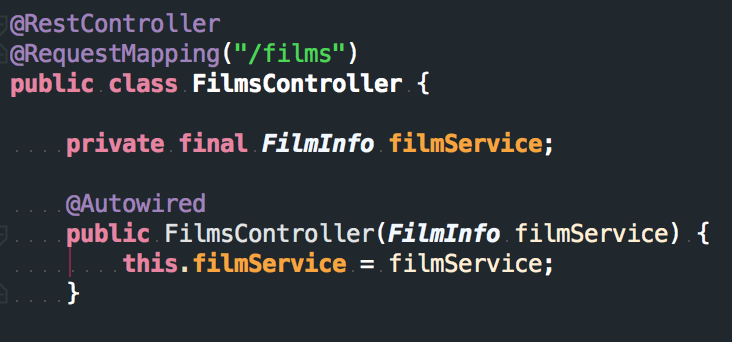
\includegraphics[width=9cm]{autowired-components}
      \caption{Spring's automatic dependency injection}
      \label{fig:spring-autowired-components}
    \end{figure}

  \subsection{Spring Hateoas}

  \subsection{Objectify}
    Objectify (\url{https://github.com/objectify/objectify}) is a JPA-like library which allows you to easily connect to Google datastore, and is the library reccomended by Google for doing so in a Java program. Previously I had built the DAO using Hibernate (\url{http://hibernate.org}), however this was not compatibile with datastore's due to non-compliance with Google's proprietary GQL language. While this worked well for what it was required to do, I ended up having to sacrifice some design points that Hibernate had previously allowed me to use. For example, with Hibernate you are able to declare class fields as ‘final’ - with objectify this is not possible as it sets the values after object initialisation.

  \subsection{Guava}
    Google Guava (\url{https://github.com/google/guava}) is a very useful set of libraries that introduce a lot of new functionality to Java. While I originally made more use of this library when I first started the application and have since refactored most uses out of the code, it is still used for array/map initialisation with a static factory, to hide the ugliness of object initialisation that can often be distracting.

  \subsection{Apache Commons Text}
    Apache Commons Text (\url{https://commons.apache.org/proper/commons-text/}) is a set of useful utility libraries dealing with Strings/text. I used this library for its ToStringBuilder class, which uses reflection to create a string representation of a java object - eliminating the need for custom ‘toString’ methods for every data object.

  \subsection{Gson}
    Google Gson (\url{https://github.com/google/gson}) is a library for automatic serialization from a java object to a JSON string. While Jackson Dataformat

  \subsection{Jackson Dataformat XML}

  \subsection{JQuery}


\section{Refactoring}

\newpage

\bibliographystyle{agsm}
\bibliography{report}

\end{document}
